\documentclass[twoside]{book}

% Packages required by doxygen
\usepackage{calc}
\usepackage{doxygen}
\usepackage{graphicx}
\usepackage[utf8]{inputenc}
\usepackage{makeidx}
\usepackage{multicol}
\usepackage{multirow}
\usepackage{textcomp}
\usepackage[table]{xcolor}

% NLS support packages
\usepackage[spanish]{babel}
% Font selection
\usepackage[T1]{fontenc}
\usepackage{mathptmx}
\usepackage[scaled=.90]{helvet}
\usepackage{courier}
\usepackage{amssymb}
\usepackage{sectsty}
\renewcommand{\familydefault}{\sfdefault}
\allsectionsfont{%
  \fontseries{bc}\selectfont%
  \color{darkgray}%
}
\renewcommand{\DoxyLabelFont}{%
  \fontseries{bc}\selectfont%
  \color{darkgray}%
}

% Page & text layout
\usepackage{geometry}
\geometry{%
  a4paper,%
  top=2.5cm,%
  bottom=2.5cm,%
  left=2.5cm,%
  right=2.5cm%
}
\tolerance=750
\hfuzz=15pt
\hbadness=750
\setlength{\emergencystretch}{15pt}
\setlength{\parindent}{0cm}
\setlength{\parskip}{0.2cm}
\makeatletter
\renewcommand{\paragraph}{%
  \@startsection{paragraph}{4}{0ex}{-1.0ex}{1.0ex}{%
    \normalfont\normalsize\bfseries\SS@parafont%
  }%
}
\renewcommand{\subparagraph}{%
  \@startsection{subparagraph}{5}{0ex}{-1.0ex}{1.0ex}{%
    \normalfont\normalsize\bfseries\SS@subparafont%
  }%
}
\makeatother

% Headers & footers
\usepackage{fancyhdr}
\pagestyle{fancyplain}
\fancyhead[LE]{\fancyplain{}{\bfseries\thepage}}
\fancyhead[CE]{\fancyplain{}{}}
\fancyhead[RE]{\fancyplain{}{\bfseries\leftmark}}
\fancyhead[LO]{\fancyplain{}{\bfseries\rightmark}}
\fancyhead[CO]{\fancyplain{}{}}
\fancyhead[RO]{\fancyplain{}{\bfseries\thepage}}
\fancyfoot[LE]{\fancyplain{}{}}
\fancyfoot[CE]{\fancyplain{}{}}
\fancyfoot[RE]{\fancyplain{}{\bfseries\scriptsize Generado el Lunes, 8 de Julio de 2013 07:16:32 para Sudoku por Doxygen }}
\fancyfoot[LO]{\fancyplain{}{\bfseries\scriptsize Generado el Lunes, 8 de Julio de 2013 07:16:32 para Sudoku por Doxygen }}
\fancyfoot[CO]{\fancyplain{}{}}
\fancyfoot[RO]{\fancyplain{}{}}
\renewcommand{\footrulewidth}{0.4pt}
\renewcommand{\chaptermark}[1]{%
  \markboth{#1}{}%
}
\renewcommand{\sectionmark}[1]{%
  \markright{\thesection\ #1}%
}

% Indices & bibliography
\usepackage{natbib}
\usepackage[titles]{tocloft}
\setcounter{tocdepth}{3}
\setcounter{secnumdepth}{5}
\makeindex

% Custom commands
\newcommand{\clearemptydoublepage}{%
  \newpage{\pagestyle{empty}\cleardoublepage}%
}


%===== C O N T E N T S =====

\begin{document}

% Titlepage & ToC
\pagenumbering{roman}
\begin{titlepage}
\vspace*{7cm}
\begin{center}%
{\Large Sudoku \\[1ex]\large 1.\-0 }\\
\vspace*{1cm}
{\large Generado por Doxygen 1.8.4}\\
\vspace*{0.5cm}
{\small Lunes, 8 de Julio de 2013 07:16:32}\\
\end{center}
\end{titlepage}
\clearemptydoublepage
\tableofcontents
\clearemptydoublepage
\pagenumbering{arabic}

%--- Begin generated contents ---
\chapter{proyecto\-\_\-lenguajes\-\_\-1er\-Parcial}
\label{md_C:_Users_Diego_Documents_GitHub_proyecto_lenguajes_1erParcial_README}
\input{md__c_1__users__diego__documents__git_hub_proyecto_lenguajes_1er_parcial__r_e_a_d_m_e}
\chapter{Indice de namespaces}
\section{Lista de 'namespaces'}
Lista de los 'namespaces', con una breve descripción\-:\begin{DoxyCompactList}
\item\contentsline{section}{{\bf Ui} }{\pageref{namespace_ui}}{}
\end{DoxyCompactList}

\chapter{Indice jerárquico}
\section{Jerarquía de la clase}
Esta lista de herencias esta ordenada aproximadamente por orden alfabético\-:\begin{DoxyCompactList}
\item Q\-Main\-Window\begin{DoxyCompactList}
\item \contentsline{section}{Cargar\-Sudoku}{\pageref{class_cargar_sudoku}}{}
\item \contentsline{section}{Guardar\-Sudoku}{\pageref{class_guardar_sudoku}}{}
\item \contentsline{section}{sudoku}{\pageref{classsudoku}}{}
\item \contentsline{section}{Ventana\-Principal}{\pageref{class_ventana_principal}}{}
\end{DoxyCompactList}
\item Q\-Widget\begin{DoxyCompactList}
\item \contentsline{section}{Puntajes}{\pageref{class_puntajes}}{}
\end{DoxyCompactList}
\end{DoxyCompactList}

\chapter{Índice de clases}
\section{Lista de clases}
Lista de las clases, estructuras, uniones e interfaces con una breve descripción\-:\begin{DoxyCompactList}
\item\contentsline{section}{{\bf Cargar\-Sudoku} }{\pageref{class_cargar_sudoku}}{}
\item\contentsline{section}{{\bf Guardar\-Sudoku} }{\pageref{class_guardar_sudoku}}{}
\item\contentsline{section}{{\bf Puntajes} }{\pageref{class_puntajes}}{}
\item\contentsline{section}{{\bf sudoku} }{\pageref{classsudoku}}{}
\item\contentsline{section}{{\bf Ventana\-Principal} }{\pageref{class_ventana_principal}}{}
\end{DoxyCompactList}

\chapter{Indice de archivos}
\section{Lista de archivos}
Lista de todos los archivos con descripciones breves\-:\begin{DoxyCompactList}
\item\contentsline{section}{{\bf cargarsudoku.\-cpp} }{\pageref{cargarsudoku_8cpp}}{}
\item\contentsline{section}{{\bf cargarsudoku.\-h} }{\pageref{cargarsudoku_8h}}{}
\item\contentsline{section}{{\bf guardarsudoku.\-cpp} }{\pageref{guardarsudoku_8cpp}}{}
\item\contentsline{section}{{\bf guardarsudoku.\-h} }{\pageref{guardarsudoku_8h}}{}
\item\contentsline{section}{{\bf main.\-cpp} }{\pageref{main_8cpp}}{}
\item\contentsline{section}{{\bf puntajes.\-cpp} }{\pageref{puntajes_8cpp}}{}
\item\contentsline{section}{{\bf puntajes.\-h} }{\pageref{puntajes_8h}}{}
\item\contentsline{section}{{\bf sudoku.\-cpp} }{\pageref{sudoku_8cpp}}{}
\item\contentsline{section}{{\bf sudoku.\-h} }{\pageref{sudoku_8h}}{}
\item\contentsline{section}{{\bf ventanaprincipal.\-cpp} }{\pageref{ventanaprincipal_8cpp}}{}
\item\contentsline{section}{{\bf ventanaprincipal.\-h} }{\pageref{ventanaprincipal_8h}}{}
\end{DoxyCompactList}

\chapter{Documentación de namespaces}
\section{Referencia del Namespace Ui}
\label{namespace_ui}\index{Ui@{Ui}}


\subsection{Descripción detallada}
C\-A\-R\-G\-A\-R\-S\-U\-D\-O\-K\-U\-\_\-\-H

P\-U\-N\-T\-A\-J\-E\-S\-\_\-\-H

S\-U\-D\-O\-K\-U\-\_\-\-H

V\-E\-N\-T\-A\-N\-A\-P\-R\-I\-N\-C\-I\-P\-A\-L\-\_\-\-H 
\chapter{Documentación de las clases}
\section{Referencia de la Clase Cargar\-Sudoku}
\label{class_cargar_sudoku}\index{Cargar\-Sudoku@{Cargar\-Sudoku}}


{\ttfamily \#include $<$cargarsudoku.\-h$>$}

Diagrama de herencias de Cargar\-Sudoku\begin{figure}[H]
\begin{center}
\leavevmode
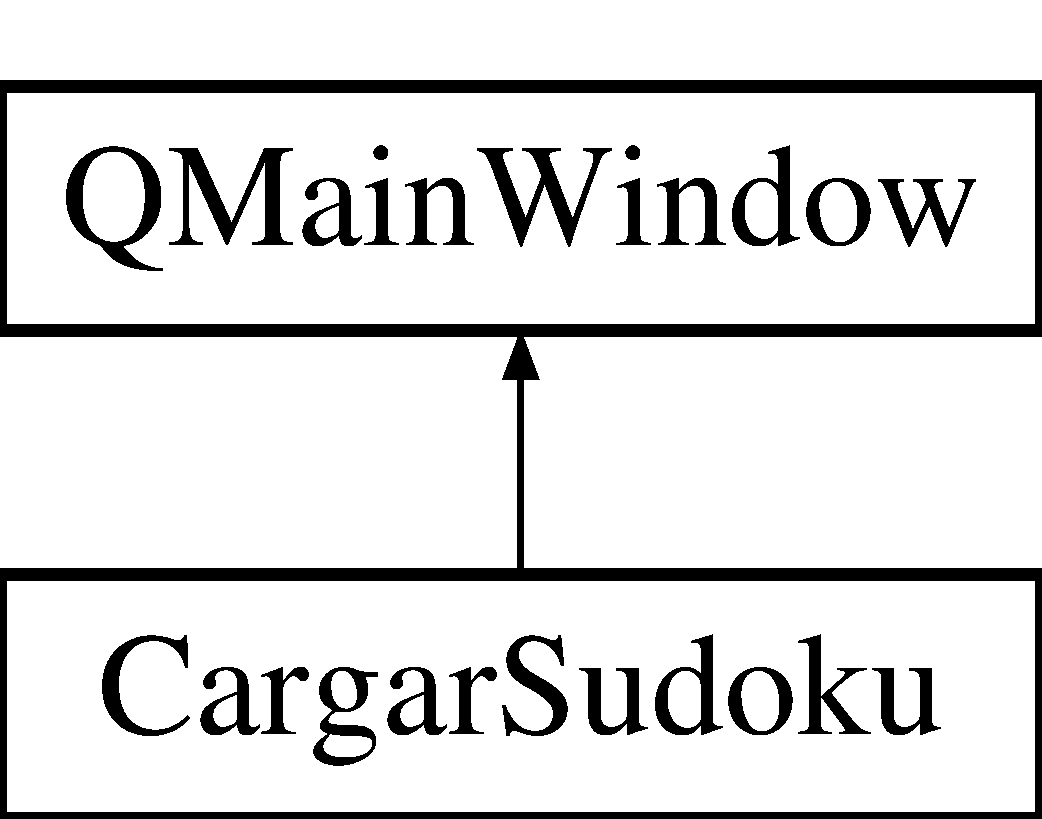
\includegraphics[height=2.000000cm]{class_cargar_sudoku}
\end{center}
\end{figure}
\subsection*{Métodos públicos}
\begin{DoxyCompactItemize}
\item 
{\bf Cargar\-Sudoku} (Q\-Widget $\ast$parent=0)
\item 
{\bf $\sim$\-Cargar\-Sudoku} ()
\item 
void {\bf set\-Combo} (Q\-Combo\-Box $\ast$combo\-C, int cont, Q\-String nombre\-J, Q\-String nivel\-J)
\end{DoxyCompactItemize}


\subsection{Documentación del constructor y destructor}
\index{Cargar\-Sudoku@{Cargar\-Sudoku}!Cargar\-Sudoku@{Cargar\-Sudoku}}
\index{Cargar\-Sudoku@{Cargar\-Sudoku}!CargarSudoku@{Cargar\-Sudoku}}
\subsubsection[{Cargar\-Sudoku}]{\setlength{\rightskip}{0pt plus 5cm}Cargar\-Sudoku\-::\-Cargar\-Sudoku (
\begin{DoxyParamCaption}
\item[{Q\-Widget $\ast$}]{parent = {\ttfamily 0}}
\end{DoxyParamCaption}
)\hspace{0.3cm}{\ttfamily [explicit]}}\label{class_cargar_sudoku_afbcf43db004504842bcb18747abaa525}

\begin{DoxyCode}
5                                           :
6     QMainWindow(parent),
7     ui(\textcolor{keyword}{new} Ui::CargarSudoku)
8 \{
9     ui->setupUi(\textcolor{keyword}{this});
10 \}
\end{DoxyCode}
\index{Cargar\-Sudoku@{Cargar\-Sudoku}!$\sim$\-Cargar\-Sudoku@{$\sim$\-Cargar\-Sudoku}}
\index{$\sim$\-Cargar\-Sudoku@{$\sim$\-Cargar\-Sudoku}!CargarSudoku@{Cargar\-Sudoku}}
\subsubsection[{$\sim$\-Cargar\-Sudoku}]{\setlength{\rightskip}{0pt plus 5cm}Cargar\-Sudoku\-::$\sim$\-Cargar\-Sudoku (
\begin{DoxyParamCaption}
{}
\end{DoxyParamCaption}
)}\label{class_cargar_sudoku_a4df0369fd0ccc87d3cb3a8420623e320}

\begin{DoxyCode}
12                            \{
13     \textcolor{keyword}{delete} ui;
14 \}
\end{DoxyCode}


\subsection{Documentación de las funciones miembro}
\index{Cargar\-Sudoku@{Cargar\-Sudoku}!set\-Combo@{set\-Combo}}
\index{set\-Combo@{set\-Combo}!CargarSudoku@{Cargar\-Sudoku}}
\subsubsection[{set\-Combo}]{\setlength{\rightskip}{0pt plus 5cm}void Cargar\-Sudoku\-::set\-Combo (
\begin{DoxyParamCaption}
\item[{Q\-Combo\-Box $\ast$}]{combo\-C, }
\item[{int}]{cont, }
\item[{Q\-String}]{nombre\-J, }
\item[{Q\-String}]{nivel\-J}
\end{DoxyParamCaption}
)}\label{class_cargar_sudoku_a1a6f8b6dff18333c1f03c2c46fb38d86}

\begin{DoxyCode}
16                                                                                        \{
17     nombreJugador = nombreJ;
18     nivelJugador = nivelJ;
19     \textcolor{keywordflow}{for}(\textcolor{keywordtype}{int} i=0; i < cont; i++)\{
20         \textcolor{keywordflow}{if}(comboC->itemText(i) != \textcolor{stringliteral}{""})
21                ui->comboBoxCargar->addItem(comboC->itemText(i));
22     \}
23 \}
\end{DoxyCode}


La documentación para esta clase fue generada a partir de los siguientes ficheros\-:\begin{DoxyCompactItemize}
\item 
{\bf cargarsudoku.\-h}\item 
{\bf cargarsudoku.\-cpp}\end{DoxyCompactItemize}

\section{Referencia de la Clase Guardar\-Sudoku}
\label{class_guardar_sudoku}\index{Guardar\-Sudoku@{Guardar\-Sudoku}}


{\ttfamily \#include $<$guardarsudoku.\-h$>$}

Diagrama de herencias de Guardar\-Sudoku\begin{figure}[H]
\begin{center}
\leavevmode
\includegraphics[height=2.000000cm]{class_guardar_sudoku}
\end{center}
\end{figure}
\subsection*{Métodos públicos}
\begin{DoxyCompactItemize}
\item 
{\bf Guardar\-Sudoku} (Q\-Widget $\ast$parent=0)
\item 
{\bf $\sim$\-Guardar\-Sudoku} ()
\end{DoxyCompactItemize}


\subsection{Documentación del constructor y destructor}
\index{Guardar\-Sudoku@{Guardar\-Sudoku}!Guardar\-Sudoku@{Guardar\-Sudoku}}
\index{Guardar\-Sudoku@{Guardar\-Sudoku}!GuardarSudoku@{Guardar\-Sudoku}}
\subsubsection[{Guardar\-Sudoku}]{\setlength{\rightskip}{0pt plus 5cm}Guardar\-Sudoku\-::\-Guardar\-Sudoku (
\begin{DoxyParamCaption}
\item[{Q\-Widget $\ast$}]{parent = {\ttfamily 0}}
\end{DoxyParamCaption}
)\hspace{0.3cm}{\ttfamily [explicit]}}\label{class_guardar_sudoku_adbb329392a24c801db21ee589ff0b103}

\begin{DoxyCode}
6                                             :
7     QMainWindow(parent),
8     ui(\textcolor{keyword}{new} Ui::GuardarSudoku)
9 \{
10     ui->setupUi(\textcolor{keyword}{this});
11 \}
\end{DoxyCode}
\index{Guardar\-Sudoku@{Guardar\-Sudoku}!$\sim$\-Guardar\-Sudoku@{$\sim$\-Guardar\-Sudoku}}
\index{$\sim$\-Guardar\-Sudoku@{$\sim$\-Guardar\-Sudoku}!GuardarSudoku@{Guardar\-Sudoku}}
\subsubsection[{$\sim$\-Guardar\-Sudoku}]{\setlength{\rightskip}{0pt plus 5cm}Guardar\-Sudoku\-::$\sim$\-Guardar\-Sudoku (
\begin{DoxyParamCaption}
{}
\end{DoxyParamCaption}
)}\label{class_guardar_sudoku_a7f107d3112be0524695b13c7ae0e8355}

\begin{DoxyCode}
12                              \{
13     \textcolor{keyword}{delete} ui;
14 \}
\end{DoxyCode}


La documentación para esta clase fue generada a partir de los siguientes ficheros\-:\begin{DoxyCompactItemize}
\item 
{\bf guardarsudoku.\-h}\item 
{\bf guardarsudoku.\-cpp}\end{DoxyCompactItemize}

\section{Referencia de la Clase Puntajes}
\label{class_puntajes}\index{Puntajes@{Puntajes}}


{\ttfamily \#include $<$puntajes.\-h$>$}

Diagrama de herencias de Puntajes\begin{figure}[H]
\begin{center}
\leavevmode
\includegraphics[height=2.000000cm]{class_puntajes}
\end{center}
\end{figure}
\subsection*{Métodos públicos}
\begin{DoxyCompactItemize}
\item 
{\bf Puntajes} (Q\-Widget $\ast$parent=0)
\item 
{\bf $\sim$\-Puntajes} ()
\item 
void {\bf set\-Puntajes} ()
\end{DoxyCompactItemize}


\subsection{Documentación del constructor y destructor}
\index{Puntajes@{Puntajes}!Puntajes@{Puntajes}}
\index{Puntajes@{Puntajes}!Puntajes@{Puntajes}}
\subsubsection[{Puntajes}]{\setlength{\rightskip}{0pt plus 5cm}Puntajes\-::\-Puntajes (
\begin{DoxyParamCaption}
\item[{Q\-Widget $\ast$}]{parent = {\ttfamily 0}}
\end{DoxyParamCaption}
)\hspace{0.3cm}{\ttfamily [explicit]}}\label{class_puntajes_af2f3d4183d995328106f6ee05c05a184}

\begin{DoxyCode}
5                                   :
6     QWidget(parent),
7     ui(\textcolor{keyword}{new} Ui::Puntajes)
8 \{
9     ui->setupUi(\textcolor{keyword}{this});
10 \}
\end{DoxyCode}
\index{Puntajes@{Puntajes}!$\sim$\-Puntajes@{$\sim$\-Puntajes}}
\index{$\sim$\-Puntajes@{$\sim$\-Puntajes}!Puntajes@{Puntajes}}
\subsubsection[{$\sim$\-Puntajes}]{\setlength{\rightskip}{0pt plus 5cm}Puntajes\-::$\sim$\-Puntajes (
\begin{DoxyParamCaption}
{}
\end{DoxyParamCaption}
)}\label{class_puntajes_a960a1c2f5cd6398440e045326d64f385}

\begin{DoxyCode}
13 \{
14     \textcolor{keyword}{delete} ui;
15 \}
\end{DoxyCode}


\subsection{Documentación de las funciones miembro}
\index{Puntajes@{Puntajes}!set\-Puntajes@{set\-Puntajes}}
\index{set\-Puntajes@{set\-Puntajes}!Puntajes@{Puntajes}}
\subsubsection[{set\-Puntajes}]{\setlength{\rightskip}{0pt plus 5cm}void Puntajes\-::set\-Puntajes (
\begin{DoxyParamCaption}
{}
\end{DoxyParamCaption}
)}\label{class_puntajes_a8e0af6587afe02db1d191ca58a41b501}

\begin{DoxyCode}
17                           \{
18     \textcolor{keywordtype}{int} bandera=0;
19     QStringList  valores;
20 
21     QString nomJugador, nivelC, crono, datosSudoku;
22     QString mFilemane = \textcolor{stringliteral}{"guardar.txt"};
23     QFile mFile(mFilemane);
24 
25     \textcolor{keywordflow}{if}(mFile.exists())\{
26 
27         mFile.open(QIODevice::Text | QIODevice::ReadOnly);
28         \textcolor{keywordflow}{if}(!mFile.isOpen())\{\textcolor{keywordflow}{return};\}
29         QTextStream txtstr(&mFile);
30 
31         \textcolor{keywordflow}{while}(!txtstr.atEnd())\{
32             datosSudoku = txtstr.readLine();
33             mFile.flush();
34             mFile.close();
35 
36             valores = datosSudoku.split(\textcolor{stringliteral}{"/"});
37             nomJugador = valores[0];
38             nivelC = valores[1];
39             crono = valores[2];
40             datosSudoku = valores[3];
41 
42             QStringList valor;
43             valor = crono.split(\textcolor{stringliteral}{":"});
44             \textcolor{keywordtype}{int} min = valor[0].toDouble(), seg = valor[1].toDouble(), mseg = valor[2].toDouble();
45             \textcolor{keywordtype}{int} puntaje = 0;
46             \textcolor{keywordflow}{if} (nivelC == \textcolor{stringliteral}{"Juvenil"})\{
47                 puntaje = 90*(min+seg+mseg)/3;
48             \}\textcolor{keywordflow}{else} \textcolor{keywordflow}{if}(nivelC == \textcolor{stringliteral}{"Profesional"})\{
49                 puntaje = 90*(min+seg+mseg)/2;
50             \}\textcolor{keywordflow}{else} \textcolor{keywordflow}{if}(nivelC == \textcolor{stringliteral}{"Experto"})\{
51                 puntaje = 90*(min+seg+mseg);
52             \}
53             QString str = QString::number(puntaje);
54             ui->textPuntajes->insertPlainText(nomJugador.toUpper()+\textcolor{stringliteral}{"\(\backslash\)t"}+nivelC+\textcolor{stringliteral}{"\(\backslash\)t"}+str+\textcolor{stringliteral}{"\(\backslash\)n"});
55             bandera = 1;
56 
57         \}
58     \}
59     \textcolor{keywordflow}{if}(bandera == 0)\{
60         ui->textPuntajes->setDisabled(\textcolor{keyword}{true});
61         QMessageBox::information(\textcolor{keyword}{this}, \textcolor{stringliteral}{"MENSAJE"}, \textcolor{stringliteral}{"No existe Puntajes\(\backslash\)nGuardados"},\textcolor{stringliteral}{"ACEPTAR"});
62 
63     \}
64 \}
\end{DoxyCode}


La documentación para esta clase fue generada a partir de los siguientes ficheros\-:\begin{DoxyCompactItemize}
\item 
{\bf puntajes.\-h}\item 
{\bf puntajes.\-cpp}\end{DoxyCompactItemize}

\section{Referencia de la Clase sudoku}
\label{classsudoku}\index{sudoku@{sudoku}}


{\ttfamily \#include $<$sudoku.\-h$>$}

Diagrama de herencias de sudoku\begin{figure}[H]
\begin{center}
\leavevmode
\includegraphics[height=2.000000cm]{classsudoku}
\end{center}
\end{figure}
\subsection*{Métodos públicos}
\begin{DoxyCompactItemize}
\item 
{\bf sudoku} (Q\-Widget $\ast$parent=0)
\item 
{\bf $\sim$sudoku} ()
\item 
void {\bf set\-Cargar} (Q\-String datos, Q\-String nivel, Q\-String cronometro, Q\-String nombre)
\item 
void {\bf obtener\-Nombre\-Nivel} (Q\-String nivel, Q\-String nombre)
\end{DoxyCompactItemize}


\subsection{Documentación del constructor y destructor}
\index{sudoku@{sudoku}!sudoku@{sudoku}}
\index{sudoku@{sudoku}!sudoku@{sudoku}}
\subsubsection[{sudoku}]{\setlength{\rightskip}{0pt plus 5cm}sudoku\-::sudoku (
\begin{DoxyParamCaption}
\item[{Q\-Widget $\ast$}]{parent = {\ttfamily 0}}
\end{DoxyParamCaption}
)\hspace{0.3cm}{\ttfamily [explicit]}}\label{classsudoku_abde738c9d12bb83ba78a4964ff2a8c9b}

\begin{DoxyCode}
10                               :
11     QMainWindow(parent),
12     ui(\textcolor{keyword}{new} Ui::sudoku)
13 \{
14     ui->setupUi(\textcolor{keyword}{this});
15     initGui();
16     timer = \textcolor{keyword}{new} QTimer(\textcolor{keyword}{this});
17 
18     connect(timer, SIGNAL(timeout()), \textcolor{keyword}{this}, SLOT(update()));
19     \textcolor{comment}{//timer->start(1000);}
20 \}
\end{DoxyCode}
\index{sudoku@{sudoku}!$\sim$sudoku@{$\sim$sudoku}}
\index{$\sim$sudoku@{$\sim$sudoku}!sudoku@{sudoku}}
\subsubsection[{$\sim$sudoku}]{\setlength{\rightskip}{0pt plus 5cm}sudoku\-::$\sim$sudoku (
\begin{DoxyParamCaption}
{}
\end{DoxyParamCaption}
)}\label{classsudoku_a53ad20f14c9c6a6c03ef42b96bfb5939}

\begin{DoxyCode}
22                \{
23     \textcolor{keyword}{delete} ui;
24 \}
\end{DoxyCode}


\subsection{Documentación de las funciones miembro}
\index{sudoku@{sudoku}!obtener\-Nombre\-Nivel@{obtener\-Nombre\-Nivel}}
\index{obtener\-Nombre\-Nivel@{obtener\-Nombre\-Nivel}!sudoku@{sudoku}}
\subsubsection[{obtener\-Nombre\-Nivel}]{\setlength{\rightskip}{0pt plus 5cm}void sudoku\-::obtener\-Nombre\-Nivel (
\begin{DoxyParamCaption}
\item[{Q\-String}]{nivel, }
\item[{Q\-String}]{nombre}
\end{DoxyParamCaption}
)}\label{classsudoku_ac7ef4c2a29416d780df2e5f969856413}
Funcion de enviar nombre y nivel 
\begin{DoxyCode}
415                                                             \{
416     nivelSudoku = nivel;
417     nombreJugador = nombre;
418     
419     ui->textJugador->setText(nombre);
420     ui->textJugador->setEnabled(\textcolor{keyword}{false});
421     ui->textNivel->setText(nivel);
422     ui->textNivel->setEnabled(\textcolor{keyword}{false});
423 \}
\end{DoxyCode}
\index{sudoku@{sudoku}!set\-Cargar@{set\-Cargar}}
\index{set\-Cargar@{set\-Cargar}!sudoku@{sudoku}}
\subsubsection[{set\-Cargar}]{\setlength{\rightskip}{0pt plus 5cm}void sudoku\-::set\-Cargar (
\begin{DoxyParamCaption}
\item[{Q\-String}]{datos, }
\item[{Q\-String}]{nivel, }
\item[{Q\-String}]{cronometro, }
\item[{Q\-String}]{nombre}
\end{DoxyParamCaption}
)}\label{classsudoku_aed73f727b9be61f82a530fbb347da182}
D\-E\-S\-E\-N\-C\-R\-I\-P\-T\-A\-R P\-A\-N\-T\-I\-L\-L\-A D\-E\-L S\-U\-D\-O\-K\-U 
\begin{DoxyCode}
69                                                                                       \{
70    QStringList  valor;
71    datosCargados = datos;
72    QStringList  valores;
73    \textcolor{keywordtype}{int} i,j,k=0;
74    \textcolor{keywordtype}{double} cont =33, opera;
75    valores = datosCargados.split(\textcolor{stringliteral}{","});
76    \textcolor{keywordflow}{for}(i = 0; i < 9; i++)\{
77        \textcolor{keywordflow}{for}(j = 0; j < 9; j++)\{
78            \textcolor{keywordflow}{if}(valores[k].toInt() == 33)\{
79                numbertext[i][j]->setDisabled(\textcolor{keyword}{false});
80                numbertext[i][j]->setText(\textcolor{stringliteral}{""});
81            \}\textcolor{keywordflow}{else}\{
83                \textcolor{keywordflow}{if}((valores[k].toInt())%2 == 0)\{
84                    opera = sqrt(valores[k].toDouble()-cont);
85                \}\textcolor{keywordflow}{else}\{
86                    opera = sqrt(2*(valores[k].toDouble()-cont));
87                \}
88                numbertext[i][j]->setTextColor(Qt::blue);
89                numbertext[i][j]->setText(QString::number(opera));
90                numbertext[i][j]->setDisabled(\textcolor{keyword}{true});
91            \}
92            numbertext[i][j]->setAlignment(Qt::AlignRight);
93            k++;
94        \}
95    \}
96    ui->textJugador->setText(nombre);
97    ui->textJugador->setEnabled(\textcolor{keyword}{false});
98    ui->textNivel->setText(nivel);
99    ui->textNivel->setEnabled(\textcolor{keyword}{false});
100 
101 
102    valor = cronometro.split(\textcolor{stringliteral}{":"});
103    \textcolor{keywordtype}{int} minutos=valor[0].toDouble(), segundos = valor[1].toDouble(), milisegundos = valor[2].toDouble();
104    min = minutos;
105    seg = segundos;
106    miliseg = milisegundos;
107 
108    timer->start(10);
109    this->show();
110 \}
\end{DoxyCode}


La documentación para esta clase fue generada a partir de los siguientes ficheros\-:\begin{DoxyCompactItemize}
\item 
{\bf sudoku.\-h}\item 
{\bf sudoku.\-cpp}\end{DoxyCompactItemize}

\section{Referencia de la Clase Ventana\-Principal}
\label{class_ventana_principal}\index{Ventana\-Principal@{Ventana\-Principal}}


{\ttfamily \#include $<$ventanaprincipal.\-h$>$}

Diagrama de herencias de Ventana\-Principal\begin{figure}[H]
\begin{center}
\leavevmode
\includegraphics[height=2.000000cm]{class_ventana_principal}
\end{center}
\end{figure}
\subsection*{Métodos públicos}
\begin{DoxyCompactItemize}
\item 
{\bf Ventana\-Principal} (Q\-Widget $\ast$parent=0)
\item 
{\bf $\sim$\-Ventana\-Principal} ()
\end{DoxyCompactItemize}
\subsection*{Métodos protegidos}
\begin{DoxyCompactItemize}
\item 
void {\bf change\-Event} (Q\-Event $\ast$e)
\end{DoxyCompactItemize}


\subsection{Documentación del constructor y destructor}
\index{Ventana\-Principal@{Ventana\-Principal}!Ventana\-Principal@{Ventana\-Principal}}
\index{Ventana\-Principal@{Ventana\-Principal}!VentanaPrincipal@{Ventana\-Principal}}
\subsubsection[{Ventana\-Principal}]{\setlength{\rightskip}{0pt plus 5cm}Ventana\-Principal\-::\-Ventana\-Principal (
\begin{DoxyParamCaption}
\item[{Q\-Widget $\ast$}]{parent = {\ttfamily 0}}
\end{DoxyParamCaption}
)}\label{class_ventana_principal_afc1895e635aa9cae6c2890882727f12b}

\begin{DoxyCode}
6                                                   :
7     QMainWindow(parent),
8     ui(\textcolor{keyword}{new} Ui::VentanaPrincipal)
9 \{
10     ui->setupUi(\textcolor{keyword}{this});
11     ui->comboBox->addItem(\textcolor{stringliteral}{"Juvenil"});
12     ui->comboBox->addItem(\textcolor{stringliteral}{"Profesional"});
13     ui->comboBox->addItem(\textcolor{stringliteral}{"Experto"});
14     timer = \textcolor{keyword}{new} QTimer(\textcolor{keyword}{this});
15 
16     connect(timer, SIGNAL(timeout()), \textcolor{keyword}{this}, SLOT(tiempoFuera()));
17 \}
\end{DoxyCode}
\index{Ventana\-Principal@{Ventana\-Principal}!$\sim$\-Ventana\-Principal@{$\sim$\-Ventana\-Principal}}
\index{$\sim$\-Ventana\-Principal@{$\sim$\-Ventana\-Principal}!VentanaPrincipal@{Ventana\-Principal}}
\subsubsection[{$\sim$\-Ventana\-Principal}]{\setlength{\rightskip}{0pt plus 5cm}Ventana\-Principal\-::$\sim$\-Ventana\-Principal (
\begin{DoxyParamCaption}
{}
\end{DoxyParamCaption}
)}\label{class_ventana_principal_aeeba538e11b05363e00e224649df9a0a}

\begin{DoxyCode}
19                                    \{
20     \textcolor{keyword}{delete} ui;
21 \}
\end{DoxyCode}


\subsection{Documentación de las funciones miembro}
\index{Ventana\-Principal@{Ventana\-Principal}!change\-Event@{change\-Event}}
\index{change\-Event@{change\-Event}!VentanaPrincipal@{Ventana\-Principal}}
\subsubsection[{change\-Event}]{\setlength{\rightskip}{0pt plus 5cm}void Ventana\-Principal\-::change\-Event (
\begin{DoxyParamCaption}
\item[{Q\-Event $\ast$}]{e}
\end{DoxyParamCaption}
)\hspace{0.3cm}{\ttfamily [protected]}}\label{class_ventana_principal_a02cdcd90f9bfddb12cd517517f3a81c2}

\begin{DoxyCode}
23                                            \{
24     QMainWindow::changeEvent(e);
25     \textcolor{keywordflow}{switch} (e->type()) \{
26     \textcolor{keywordflow}{case} QEvent::LanguageChange:
27         ui->retranslateUi(\textcolor{keyword}{this});
28         \textcolor{keywordflow}{break};
29     \textcolor{keywordflow}{default}:    \textcolor{keywordflow}{break};
30     \}
31 \}
\end{DoxyCode}


La documentación para esta clase fue generada a partir de los siguientes ficheros\-:\begin{DoxyCompactItemize}
\item 
{\bf ventanaprincipal.\-h}\item 
{\bf ventanaprincipal.\-cpp}\end{DoxyCompactItemize}

\chapter{Documentación de archivos}
\section{Referencia del Archivo cargarsudoku.\-cpp}
\label{cargarsudoku_8cpp}\index{cargarsudoku.\-cpp@{cargarsudoku.\-cpp}}
{\ttfamily \#include \char`\"{}cargarsudoku.\-h\char`\"{}}\\*
{\ttfamily \#include \char`\"{}ui\-\_\-cargarsudoku.\-h\char`\"{}}\\*
{\ttfamily \#include \char`\"{}sudoku.\-h\char`\"{}}\\*

\section{Referencia del Archivo cargarsudoku.\-h}
\label{cargarsudoku_8h}\index{cargarsudoku.\-h@{cargarsudoku.\-h}}
{\ttfamily \#include $<$Q\-Main\-Window$>$}\\*
{\ttfamily \#include $<$Q\-File$>$}\\*
{\ttfamily \#include $<$Q\-Message\-Box$>$}\\*
{\ttfamily \#include $<$Q\-String$>$}\\*
{\ttfamily \#include $<$Q\-Text\-Stream$>$}\\*
{\ttfamily \#include $<$Q\-Combo\-Box$>$}\\*
{\ttfamily \#include \char`\"{}sudoku.\-h\char`\"{}}\\*
\subsection*{Clases}
\begin{DoxyCompactItemize}
\item 
class {\bf Cargar\-Sudoku}
\end{DoxyCompactItemize}
\subsection*{Namespaces}
\begin{DoxyCompactItemize}
\item 
{\bf Ui}
\end{DoxyCompactItemize}
\subsection*{Constant Groups}
\begin{DoxyCompactItemize}
\item 
{\bf Ui}
\end{DoxyCompactItemize}

\section{Referencia del Archivo guardarsudoku.\-cpp}
\label{guardarsudoku_8cpp}\index{guardarsudoku.\-cpp@{guardarsudoku.\-cpp}}
{\ttfamily \#include \char`\"{}guardarsudoku.\-h\char`\"{}}\\*
{\ttfamily \#include \char`\"{}ui\-\_\-guardarsudoku.\-h\char`\"{}}\\*
{\ttfamily \#include $<$math.\-h$>$}\\*

\section{Referencia del Archivo guardarsudoku.\-h}
\label{guardarsudoku_8h}\index{guardarsudoku.\-h@{guardarsudoku.\-h}}
{\ttfamily \#include $<$Q\-Main\-Window$>$}\\*
{\ttfamily \#include $<$Q\-File$>$}\\*
{\ttfamily \#include $<$Q\-Message\-Box$>$}\\*
{\ttfamily \#include $<$Q\-String$>$}\\*
{\ttfamily \#include $<$Q\-Text\-Stream$>$}\\*
\subsection*{Clases}
\begin{DoxyCompactItemize}
\item 
class {\bf Guardar\-Sudoku}
\end{DoxyCompactItemize}
\subsection*{Namespaces}
\begin{DoxyCompactItemize}
\item 
{\bf Ui}
\end{DoxyCompactItemize}
\subsection*{Constant Groups}
\begin{DoxyCompactItemize}
\item 
{\bf Ui}
\end{DoxyCompactItemize}

\section{Referencia del Archivo main.\-cpp}
\label{main_8cpp}\index{main.\-cpp@{main.\-cpp}}
{\ttfamily \#include \char`\"{}sudoku.\-h\char`\"{}}\\*
{\ttfamily \#include \char`\"{}ventanaprincipal.\-h\char`\"{}}\\*
{\ttfamily \#include $<$Q\-Application$>$}\\*
\subsection*{Funciones}
\begin{DoxyCompactItemize}
\item 
int {\bf main} (int argc, char $\ast$argv[$\,$])
\end{DoxyCompactItemize}


\subsection{Documentación de las funciones}
\index{main.\-cpp@{main.\-cpp}!main@{main}}
\index{main@{main}!main.cpp@{main.\-cpp}}
\subsubsection[{main}]{\setlength{\rightskip}{0pt plus 5cm}int main (
\begin{DoxyParamCaption}
\item[{int}]{argc, }
\item[{char $\ast$}]{argv[$\,$]}
\end{DoxyParamCaption}
)}\label{main_8cpp_a0ddf1224851353fc92bfbff6f499fa97}

\begin{DoxyCode}
6 \{
7     QApplication a(argc, argv);
8     \textcolor{comment}{//a.setStyle("fusion");}
9     VentanaPrincipal w;
10     w.show();
11     
12     \textcolor{keywordflow}{return} a.exec();
13 \}
\end{DoxyCode}

\section{Referencia del Archivo puntajes.\-cpp}
\label{puntajes_8cpp}\index{puntajes.\-cpp@{puntajes.\-cpp}}
{\ttfamily \#include \char`\"{}puntajes.\-h\char`\"{}}\\*
{\ttfamily \#include \char`\"{}ui\-\_\-puntajes.\-h\char`\"{}}\\*
{\ttfamily \#include $<$Q\-String$>$}\\*

\section{Referencia del Archivo puntajes.\-h}
\label{puntajes_8h}\index{puntajes.\-h@{puntajes.\-h}}
{\ttfamily \#include $<$Q\-Widget$>$}\\*
{\ttfamily \#include \char`\"{}ventanaprincipal.\-h\char`\"{}}\\*
\subsection*{Clases}
\begin{DoxyCompactItemize}
\item 
class {\bf Puntajes}
\end{DoxyCompactItemize}
\subsection*{Namespaces}
\begin{DoxyCompactItemize}
\item 
{\bf Ui}
\end{DoxyCompactItemize}
\subsection*{Constant Groups}
\begin{DoxyCompactItemize}
\item 
{\bf Ui}
\end{DoxyCompactItemize}

\input{_r_e_a_d_m_e_8md}
\section{Referencia del Archivo sudoku.\-cpp}
\label{sudoku_8cpp}\index{sudoku.\-cpp@{sudoku.\-cpp}}
{\ttfamily \#include \char`\"{}sudoku.\-h\char`\"{}}\\*
{\ttfamily \#include \char`\"{}ui\-\_\-sudoku.\-h\char`\"{}}\\*
{\ttfamily \#include $<$math.\-h$>$}\\*
{\ttfamily \#include $<$iostream$>$}\\*
{\ttfamily \#include $<$Q\-Char$>$}\\*

\section{Referencia del Archivo sudoku.\-h}
\label{sudoku_8h}\index{sudoku.\-h@{sudoku.\-h}}
{\ttfamily \#include $<$Q\-Main\-Window$>$}\\*
{\ttfamily \#include \char`\"{}cargarsudoku.\-h\char`\"{}}\\*
{\ttfamily \#include $<$Q\-Text\-Edit$>$}\\*
{\ttfamily \#include $<$Q\-Message\-Box$>$}\\*
{\ttfamily \#include $<$Q\-Combo\-Box$>$}\\*
{\ttfamily \#include $<$Q\-Time$>$}\\*
{\ttfamily \#include $<$Q\-Timer$>$}\\*
{\ttfamily \#include $<$Q\-Widget$>$}\\*
\subsection*{Clases}
\begin{DoxyCompactItemize}
\item 
class {\bf sudoku}
\end{DoxyCompactItemize}
\subsection*{Namespaces}
\begin{DoxyCompactItemize}
\item 
{\bf Ui}
\end{DoxyCompactItemize}
\subsection*{Constant Groups}
\begin{DoxyCompactItemize}
\item 
{\bf Ui}
\end{DoxyCompactItemize}

\section{Referencia del Archivo ventanaprincipal.\-cpp}
\label{ventanaprincipal_8cpp}\index{ventanaprincipal.\-cpp@{ventanaprincipal.\-cpp}}
{\ttfamily \#include \char`\"{}ventanaprincipal.\-h\char`\"{}}\\*
{\ttfamily \#include \char`\"{}ui\-\_\-ventanaprincipal.\-h\char`\"{}}\\*
{\ttfamily \#include \char`\"{}sudoku.\-h\char`\"{}}\\*

\section{Referencia del Archivo ventanaprincipal.\-h}
\label{ventanaprincipal_8h}\index{ventanaprincipal.\-h@{ventanaprincipal.\-h}}
{\ttfamily \#include $<$Q\-Main\-Window$>$}\\*
{\ttfamily \#include $<$Q\-Timer$>$}\\*
{\ttfamily \#include \char`\"{}sudoku.\-h\char`\"{}}\\*
{\ttfamily \#include $<$Q\-Message\-Box$>$}\\*
{\ttfamily \#include $<$puntajes.\-h$>$}\\*
\subsection*{Clases}
\begin{DoxyCompactItemize}
\item 
class {\bf Ventana\-Principal}
\end{DoxyCompactItemize}
\subsection*{Namespaces}
\begin{DoxyCompactItemize}
\item 
{\bf Ui}
\end{DoxyCompactItemize}
\subsection*{Constant Groups}
\begin{DoxyCompactItemize}
\item 
{\bf Ui}
\end{DoxyCompactItemize}

%--- End generated contents ---

% Index
\newpage
\phantomsection
\addcontentsline{toc}{part}{Índice}
\printindex

\end{document}
